\section{Campo magnetico}

\subsection{Forza di Lorentz}
La forza di Lorentz descrive una particella carica $q$ con velocità
$\vec{v}$ e un campo vettoriale $\vec{B}$
\begin{equation}
    \vec{F} q\vec{v}\times\vec{B}
\end{equation}
che generano la forza magnetica.

L'andamento delle forze segue la regola della mano destra:
\begin{figure}[H]
    \centering
    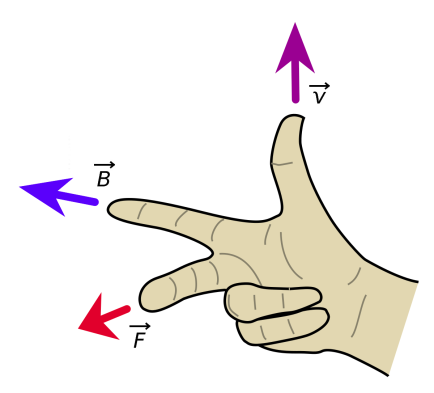
\includegraphics[width=0.2\linewidth]{imgs/12 - lorentz.png}
    \label{fig:regola_mano_destra}
    \caption{Regola mano destra}
\end{figure}

Per q positiva, la forza segue il verso di F(freccia in rosso), altrimenti ha verso opposto.

L'intensità della forza è:
\begin{equation}
    F = |qvB\sin\theta|
\end{equation}
NB:
\begin{itemize}
    \item per carica in quiete, forza = 0
    \item se v ed f solo paralleli o opposti, forza = 0
\end{itemize}

L'unità di misura è il $[T]$(Tesla), però il tesla è molto grande come unità 
di misura, perciò spesso si usa il \textbf{gauss},
$1G = 10^{-4}T$.

\subsection{Forza su un conduttore percorso da corrente}
Prima si deve ricavare il numero di portatori di carica:
\begin{equation*}
    N = nAl
\end{equation*}
dove si moltiplicano il numero dei portatoridi carica n per il volume del segmento.
La froza magnetica totale agente sulla carica $Nq$ è:
\begin{equation}
    \vec{F} = Nq\vec{v_d}\times\vec{B} = nAlq\vec{v_d}\times\vec{B}
\end{equation}

Per trovare la l'intensità della forza posso usare:
\begin{equation}
    F = IlB\sin\theta
\end{equation}

Però visto che questa frmula vale solo con fili rettilinei e campi magnetici
uniformi, bisogna integrare per ottenere il risultato nel mondo reale:
\begin{equation}
    \vec{F} = \int{Id\vec{l}\times\vec{B}}
\end{equation}

\subsection{Momento agente su una spira}
Il campo di induzione magnetica esercita una forza sul filo percorso
da corrente, può produrre un momento.

Il momento su una spira è:
\begin{equation}
    \tau = ISB\sin\theta
\end{equation}
\begin{itemize}
    \item I = corrente
    \item S = supericie
    \item B = intensità campo di induzione
    \item $\theta$ = angoolo fra vettore superficie e vettore del campo magnetico
\end{itemize}

Se invece, si ha una bobina, bisogna considerare il numero delle spire:
\begin{equation}
    \tau = NISB\sin\theta
\end{equation}
Dove N è il numero delle spire.

\subsection{Moto di cariche in presenza di campi}
La forza totale che agisce su una particella con carica q
e velocità v:
\begin{equation}
    \vec{F} = q\vec{E} + q\vec{v}\times\vec{B}
\end{equation}

Il raggio della traiettoria che assume la particella è:
\begin{equation}
    r = \frac{mv}{qB}
\end{equation}

La velocità angolare è:
\begin{equation}
    \omega = \frac{v}{r}=\frac{q}{m}B
\end{equation}